% !TEX encoding = UTF-8 Unicode

\documentclass{article}
\usepackage[french]{babel}
\author{Louis DESVERNOIS, Alexis SCHOENN, Philippe DUBOIS}
\title{%
    SAÉ24: Réseau \\
    \large Groupe 13}
% \date{9 Juin 2022}
\usepackage[left=2.5cm,right=2.5cm,top=2.5cm,bottom=2.5cm]{geometry}
\usepackage{subcaption}
\usepackage{listings}
\usepackage{minted}
\usepackage{graphicx}
\usepackage[T1]{fontenc}
\usepackage[colorlinks=true,linkcolor=black,anchorcolor=black,citecolor=black,filecolor=black,menucolor=black,runcolor=black,urlcolor=black]{hyperref}
%\setcounter{tocdepth}{1} % pour la profondeur de la ToC

\usepackage{fancyhdr}
\pagestyle{fancy}
\fancyhf{}
\renewcommand{\headrulewidth}{0pt}
\rfoot{\thepage}
\lfoot{SAÉ24: Groupe 13}

\renewcommand{\listoflistingscaption}{Table des codes}
\renewcommand{\listingscaption}{Code}

\begin{document}

\maketitle
\tableofcontents
\listoffigures
\listoflistings

\newpage
\section{Création des VLAN et routage inter-VLAN}
\subsection{VLANs}
Pour commencer nous avons dû créer quatre VLAN sur notre switch ainsi que de mettre en place le routage inter-VLAN. 
Nous avons donc d'abord créé ces VLAN avec les commandes ci-dessous.
\begin{listing}[H]
    \begin{minted}[breaklines]{text}
Switch(config)#int range fastEthernet 0/1-4
Switch(config-if-range)#sw mode access 
Switch(config-if-range)#sw access vlan 10
% Access VLAN does not exist. Creating vlan 10
    \end{minted}
    \caption{Création d'un VLAN}
    \label{reseau:switch:vlans}
\end{listing}
Nous avons répété les commandes en code \ref{reseau:switch:vlans} quatre fois en utilisant quatre interfaces par VLAN ainsi que les numéros 10, 20, 30 et 40. 
Nous avons ensuite donné des noms à ces VLAN avec les commandes \verb|vlan <no>| puis \verb|name <nom>| en mode configuration.

\begin{listing}[H]
    \begin{minted}[breaklines]{text}
VLAN Name                             Status    Ports
---- -------------------------------- --------- -------------------------------
1    default                          active    Fa0/17, Fa0/18, Fa0/19, Fa0/20
                                                Fa0/21, Fa0/22, Fa0/23, Fa0/24
                                                Gig0/1, Gig0/2
10   voix                             active    Fa0/1, Fa0/2, Fa0/3, Fa0/4
20   users                            active    Fa0/5, Fa0/6, Fa0/7, Fa0/8
30   server                           active    Fa0/9, Fa0/10, Fa0/11, Fa0/12
40   admin                            active    Fa0/13, Fa0/14, Fa0/15, Fa0/16
1002 fddi-default                     active    
1003 token-ring-default               active    
1004 fddinet-default                  active    
1005 trnet-default                    active    
    \end{minted}
    \caption{Résultats de "sh vlan brief"}
    \label{reseau:switch:sh-vlan}
\end{listing}

\subsection{Routage inter-VLAN}
Une fois les VLAN correctement crées, nous avons besoin de configurer le routage inter-VLAN en utilisant l'encapsulation dot1Q.
Pour cela, sur notre switch, nous avons choisi le port \verb|Fa0/24| comme port trunk.
\begin{listing}[H]
    \begin{minted}[breaklines]{text}
Switch(config)#int fastEthernet 0/24
Switch(config-if)#sw mode trunk 
Switch(config-if)#sw trunk allowed vlan 10,20,30,40
    \end{minted}
    \caption{Configuration du port trunk}
    \label{reseau:switch:trunk}
\end{listing}
Le trunk étant activé, nous pouvons à présent créer les interfaces virtuelles sur le routeur. Nous avons besoin d'en créer quatre, une par VLAN. 
Au niveau de nos adresses IP, étant le groupe 13, nous pouvons utiliser les réseaux \verb|172.113.x.0/24| avec \verb|x| le numéro de VLAN. Les adresses choisies pour les gateways et les SVI seront respectivement la dernière et l'avant-dernière adresse de chaque réseau.
\begin{listing}[H]
    \begin{minted}[breaklines]{text}
interface FastEthernet0/0
    no ip address
!
interface FastEthernet0/0.10
    encapsulation dot1Q 10
    ip address 172.113.10.254 255.255.255.0
!
interface FastEthernet0/0.20
    encapsulation dot1Q 20
    ip address 172.113.20.254 255.255.255.0
!
interface FastEthernet0/0.30
    encapsulation dot1Q 30
    ip address 172.113.30.254 255.255.255.0
!
interface FastEthernet0/0.40
    encapsulation dot1Q 40
    ip address 172.113.40.254 255.255.255.0
    \end{minted}
    \caption{Création des interfaces virtuelles sur le routeur}
    \label{router:sub-int}
\end{listing}
Nous pouvons également en profiter pour configurer l'interface connectée à Internet en DHCP avec la commande \verb|ip address dhcp| en mode configuration d'interface.
\begin{figure}[H]
    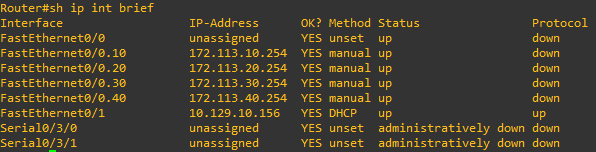
\includegraphics[width=\linewidth]{fig/router-dhcp.png}
    \caption{sh ip int brief}
    \label{router:shipintbrief}
\end{figure}
Comme nous pouvons le voir en Figure \ref{router:shipintbrief}, le routeur à bien récupéré une adresse IP avec DHCP et nous interfaces virtuelles ont correctement été configurées\footnote{Le protocole et en "down" sur Fa0/0 car au moment de la prise de la capture d'écran, un câble cassé étais utilisé}.
\newpage
\section{Mise en place du NAT et ACL}
\subsection{NAT}
Comme nous désirons utiliser Internet sur notre réseau, il est necéssaire de mettre en place un NAT. Pour cela, nous avons d'abord besoin de spécifier quelles interfaces se situent à l'intérieur du NAT et lequelles sont à l'extérieur.
Nous allons exécuter la commandes \verb|ip nat inside| sur toutes les interfaces virtuelles et la commande \verb|ip nat outside|. Ensuite, il est necéssaire de créer un ACL "permit" avec toutes les adresses source qui seront traduites par le routeur.
\begin{listing}[H]
    \begin{minted}[breaklines]{text}
Router(config)#ip access-list standard NAT
Router(config-std-nacl)#permit 172.113.0.0 0.0.255.255
Router(config-std-nacl)#exit
Router(config)#int fastEthernet 0/0.10
Router(config-subif)#ip nat inside
Router(config-subif)#int fastEthernet 0/0.20
Router(config-subif)#ip nat inside
Router(config-subif)#int fastEthernet 0/0.30
Router(config-subif)#ip nat inside
Router(config-subif)#int fastEthernet 0/0.40
Router(config-subif)#ip nat inside
Router(config-subif)#exit
Router(config)#ip nat inside source list NAT interface fastEthernet 0/1
    \end{minted}
    \caption{Configuration du NAT}
    \label{router:nat}
\end{listing}
Une fois les commandes en code \ref{router:nat} sont exécutées et que les interfaces des PC sont correctement configurées, nous devrons être capables de nous connecter à Internet sur notre réseau.
\subsection{DHCP}
Maintenant que notre NAT est mis en place, il serait intéressant de configurer le DHCP dans notre réseau.
Pour cela, nous allons utiliser notre Switch, qui est capable d'agir en tant que serveur DHCP.
\begin{listing}[H]
    \begin{minted}[breaklines]{text}
Switch(config)#ip dhcp excluded-address 172.113.20.254
Switch(config)#ip dhcp excluded-address 172.113.40.254
Switch(dhcp-config)#ip dhcp pool vlan20
Switch(dhcp-config)#network 172.113.20.0 255.255.255.0
Switch(dhcp-config)#default-router 172.113.20.254
Switch(dhcp-config)#ip dhcp pool vlan40
Switch(dhcp-config)#network 172.113.40.0 255.255.255.0
Switch(dhcp-config)#default-router 172.113.40.254
    \end{minted}
    \caption{Configuration du DHCP}
    \label{switch:dhcp}
\end{listing}
Les VLAN 10 et 30 ne sont pas configurés, car ceux-ci ne doivent pas utiliser le DHCP, en effet le DHCP du PABX présent sur le VLAN 10 entre en conflit et les serveurs du VLAN 30 sont configurés en statique.
\end{document}